% !TEX root=../master.tex

\chapter{Introduction}
\label{chp:introduction}

\section{Problem Statement}
As multirotor unmanned aerial vehicles (UAVs) have become popular
platforms for commercial and consumer products over the past decade, a variety
of new use cases have emerged that require operation from moving vehicles.
Such use cases include
maritime surveillance, package delivery, and convoy
support (see~\figref{fig:drone_convoy_support}). While there are
many facets to operating from moving vehicles, this thesis works toward creating
a robust solution to autonomously landing multirotor UAVs onto moving vehicles
in challenging conditions.

\begin{figure}[h]
  \centering
  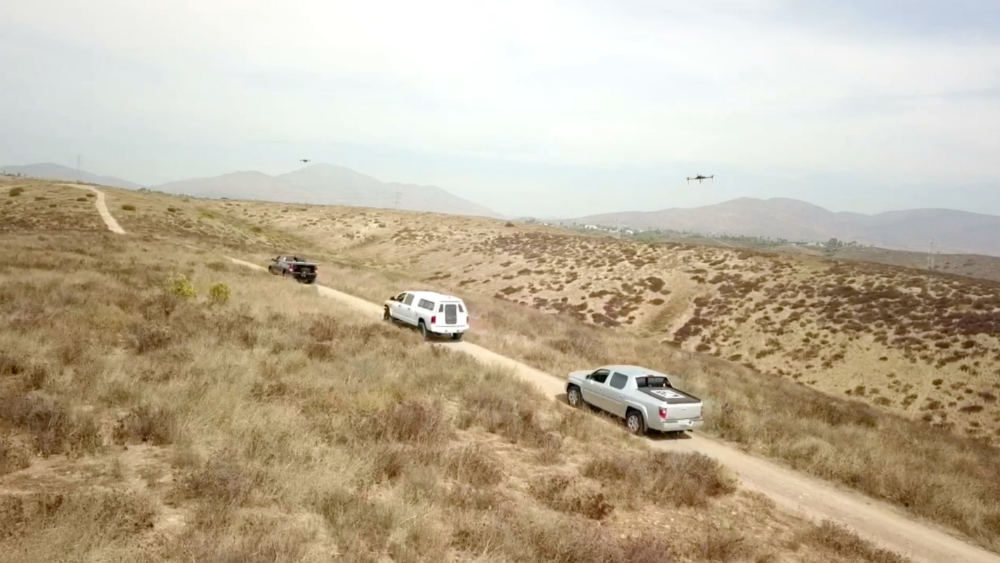
\includegraphics[width=4.5in]{figures/drone_convoy_support.png}
  \caption[UAV Convoy Support]{An example of multirotor UAVs used to increase
  situational awareness for a convoy of
vehicles~\cite{ground_vehicle_based_drones}.}
%
  \label{fig:drone_convoy_support}
\end{figure}

State-of-the-art autonomous vehicle systems require robust solutions to three
problems: state estimation, motion planning and control. In this thesis,
we propose solutions to two of those three problems, state estimation and
control, for a multirotor UAV landing on a moving vehicle.
% We leave the problem
% of motion planning as future work, providing some suggested direction
% in~\secref{sec:future_work}.

\section{Background}

While autonomous landing of multirotor UAVs onto moving vehicles has been
demonstrated in a variety of scenarios~\cite{wynn2019visual}, many problems still remain to
create a truly robust solution. Here we detail several of these outstanding
problems as they relate to the specifc fields of state estimation, control and
motion planning.

\subsection{State Estimation}
Most low-cost landing methods assume that the landing vehicle is equipped with a
fiducial marker, such as that shown in~\figref{fig:aruco_tag}, that serves as
the designated landing pad for the UAV.
In these methods, a camera mounted to the UAV detects the fiducial landing marker, providing
information about the relative position of the UAV to the landing
vehicle~\cite{borowczyk2017autonomous}. These measurements are often used in a
filtering framework, such as a Kalman filter~\cite{kalman}, to produce a
continous estimate of the relative state between the UAV and the landing
vehicle. However, during landing, it is likely
that the fiducial marker is not detected for periods of time due to occlusion,
sun glare, or UAV motion. For this reason, it is important that the relative
motion between the landing vehicle and the UAV is modeled and used to predict
the relative state when the fiducial marker is not detected.
Even with a good model though,
these methods quickly fail when the fiducial landing
marker is not detected for several seconds~\cite{ling2014precision}.

\begin{figure}[h]
  \centering
  
\includegraphics[width=2.5in]{figures/aruco_104.png}
  \caption[Visual Fiducial Landing Marker]{Visual fiducial markers such as this
    ArUco tag~\cite{garrido2016generation} are commonly used to assist in the
  landing of multirotor UAVs onto moving vehicles.}
  \label{fig:aruco_tag}
\end{figure}

When landing in challenging conditions such as strong winds, bright sun, or
dense fog, it is very common that the fiducial marker may be undetected by the UAV
for long periods of time. Therefore, to create a truly robust landing solution,
the state estimation solution must maintain an accurate estimate of the relative
state between the UAV and the landing vehicle when the fiducial landing marker
is not detected for significant durations. Chapter~\ref{chp:estimation_paper}
describes an estimation algorithm, based on the error-state Kalman
filter~\cite{roumeliotis1999circumventing}, that tracks and estimates the locations of
visual features on the landing vehicle to achieve this goal.

Visual feature
tracking and estimation is a common technique in the field of visual
odometry~\cite{qin2018vins}, however, almost all implementations assume that the
tracked visual features are static with respect to an inertial reference frame.
In the landing scenario, the landing vehicle occupies progressively more of the
field of view of the UAV's camera as the UAV descends. We also note that in most
applications, more precise state estimates are required the closer the UAV gets
to the landing vehicle. For these reasons, the described estimation algorithm
only tracks and estimates visual features that are rigidly attached to the landing vehicle.
Experimental results
from both simulation and hardware demonstrate accurate and consistent estimates
result from the proposed algorithm even when the fiducial marker is undetected
for long periods of time.

\subsection{Control}
A wide variety of control schemes for multirotor UAVs have been presented over
the past two decades. While many of these control algorithms may satisfy the
requirements for robust landing on moving vehicles, there has recently been a
movement in the robotics community to appropriately deal with the evolution of a
robot's state along a manifold using Lie theory~\cite{sola2018micro}. Though
these methods have been widely used in the field of state
estimation~\cite{sola2017quaternion, koch2017relative}, there has not been much
work done applying Lie theory to optimal control.

A controller for robustly landing a UAV onto a moving vehicle would ideally be able to
closely track a time-dependent trajectory. This would allow the UAV to
accurately land on the moving vehicle at the precise time planned by the motion
planning algorithm. To achieve this, Chapter~\ref{chp:control_paper} derives a
linear-quadratic regulator (LQR) using Lie theory and shows in both simulation
and hardware experiements that it can be used to accurately track a
time-dependent trajectory.

\subsection{Motion Planning}
The motion planning problem associated with autonomous vehicles is especially
important when it is not only important the destination the vehicle must reach,
but also the path it must take to get there. This is commonly important when
navigating around obstacles. In the case of landing on moving vehicles, motion
planning is important to assure that the UAV descends vertically on the
landing pad to avoid potential obstacles including buildings, terrain, and
vehicle superstructure.

As with the control problem, much work has been previously presented that would
likely satisfy the requirements for a robust landing
solution~\cite{mellinger2011minimum}. Solutions have also been specifically
presented to generate paths for a UAV landing on a moving
vehicle using model-predictive control in real time~\cite{baca2019autonomous}.
While we do not propose any improvements to these methods in this thesis, we
describe some potential directions for future work in~\secref{sec:future_work}.

\section{Contributions}
The research described in this thesis makes two significant contributions:
\begin{itemize}
\item A method of state estimation is developed that maintains accurate and
  consistent estimates of the state of a landing vehicle even when a fiducial landing
  marker is not detected for significant periods of time by a multirotor UAV.
\item An optimal control scheme for a multirotor UAV is derived in an error-state, linear
  quadratic regulator (LQR) formulation. This provides an optimal control scheme
  for a multirotor to follow any dynamically feasible, time-dependent
  trajectory.
\end{itemize}

These contributions were demonstrated in both simulation and hardware
results found in Chapters~\ref{chp:estimation_paper}
and~\ref{chp:control_paper}. These results give us reason to believe that a
complete and robust landing solution could be created by combining the proposed
state estimation and control schemes with a competent motion planner.

\section{Outline}

The remainder of this thesis is organized as follows.
Chapter~\ref{chp:experimental_apparatus} details the hardware and software
systems used
in the experiments. Chapter~\ref{chp:estimation_paper} describes the state
estimation algorithm that maintains accurate and consistent estimates even when
a fiducial landing marker is not detected for significant periods of time.
Chapter~\ref{chp:control_paper} derives an error-state LQR controller for a
multirotor UAV following a dynamically feasible, time-dependent trajectory.
Chapter~\ref{chp:conclusion} provides some concluding remarks including
suggestions for future work that can build upon the work described in this
thesis.
